\chapter{Hardware Architecture}

\section{Hardware inventory}

The current RUDRAv4 hardware is a modular base-control stack. The NUC is the central computer, but the low-level I/O remains distributed so that each device does what it is good at.

\begin{longtable}{p{0.22\linewidth}p{0.20\linewidth}p{0.48\linewidth}}
\toprule
Hardware & Interface to NUC or base & Engineering role\\
\midrule
Intel NUC & USB, Ethernet/Wi-Fi, DC input & Runs Ubuntu, ROS 2, launch files, bridge nodes, LiDAR driver overlays, monitoring, and development tools.\\
Mini-Box DCDC-USB & DC input/output and USB status & Regulates the NUC power rail and exposes voltage/status telemetry.\\
Arduino Uno & USB serial at 115200 baud & Reads PS2 receiver and publishes joystick packets.\\
PS2 controller/receiver & PS2X digital pins to Uno & Wireless manual driving and guard latch control.\\
Teensy 4.1 & USB serial at 115200 baud; Serial1 packet serial at 9600 baud & Converts NUC drive packets into Sabertooth packet serial and optional IMU/odometry telemetry.\\
Two Sabertooth drivers & Single-wire packet serial from Teensy TX1 & Right side address 128, left side address 129. Drives four motors as two differential sides.\\
YDLIDAR G2B & CP2102 USB serial adapter & Publishes 360-degree planar laser scans for obstacle guard and future SLAM.\\
MPU6050 & I2C to Teensy & Raw acceleration and gyro telemetry for localization experiments.\\
Wheel encoders & Interrupt pins to Teensy & Wheel-speed and odometry telemetry.\\
\bottomrule
\end{longtable}

\section{Physical and logical separation}

The architecture deliberately separates four domains:

\begin{enumerate}
  \item \textbf{Human input}: the PS2 receiver is on the Uno. If controller code changes, the Teensy motor driver firmware does not need to change.
  \item \textbf{Drive actuation}: the Teensy owns packet serial to the Sabertooths. The NUC never talks directly to the Sabertooth bus.
  \item \textbf{ROS intelligence}: the NUC owns topics, launch files, parameters, LiDAR processing, localization, and logging.
  \item \textbf{Power health}: DCDC-USB is monitored independently from the drivetrain power path.
\end{enumerate}

\begin{figure}[htbp]
\centering
\resizebox{0.98\linewidth}{!}{\begin{tikzpicture}[node distance=7mm and 10mm]
\node[rudraHw] (controller) {PS2\\controller};
\node[rudraHw,right=of controller] (receiver) {PS2 receiver\\to Uno pins};
\node[rudraHw,right=of receiver] (uno) {Arduino Uno\\PS2X};
\node[rudraBlock,right=of uno] (ros) {NUC ROS 2\\bridges};
\node[rudraHw,right=of ros] (teensy) {Teensy 4.1\\Serial1 TX};
\node[rudraHw,above right=of teensy] (right) {Right\\Sabertooth\\addr 128};
\node[rudraHw,below right=of teensy] (left) {Left\\Sabertooth\\addr 129};
\node[rudraHw,right=of right] (rm) {right motors};
\node[rudraHw,right=of left] (lm) {left motors};
\draw[rudraArrow] (controller) -- (receiver);
\draw[rudraArrow] (receiver) -- (uno);
\draw[rudraArrow] (uno) -- node[above=0.5]{USB \cmd{J,...}} (ros);
\draw[rudraArrow] (ros) -- node[above=0.5]{USB \cmd{D,...}} (teensy);
\draw[rudraArrow] (teensy) -- node[above=0.5,sloped]{packet serial} (right);
\draw[rudraArrow] (teensy) -- node[below=0.5,sloped]{same bus} (left);
\draw[rudraArrow] (right) -- (rm);
\draw[rudraArrow] (left) -- (lm);
\end{tikzpicture}}
\caption{RUDRAv4 hardware command chain from operator input to motor actuation.}
\end{figure}

\section{Known pin and address conventions}

The PS2 receiver remains wired to the Uno with the validated pinout:

\begin{center}
\begin{tabular}{lc}
\toprule
PS2 signal & Uno pin\\
\midrule
CLK & 9\\
CMD & 7\\
ATT & 6\\
DAT & 8\\
\bottomrule
\end{tabular}
\end{center}

The Sabertooth packet serial convention is:

\begin{center}
\begin{tabular}{lc}
\toprule
Device & Value\\
\midrule
Right Sabertooth address & 128\\
Left Sabertooth address & 129\\
Sabertooth packet serial baud & 9600\\
Teensy serial port to Sabertooth & \cmd{Serial1/TX1}\\
Command range & -127 to +127\\
\bottomrule
\end{tabular}
\end{center}

\begin{figure}[htbp]
\centering
\begin{subfigure}{0.46\linewidth}
\centering
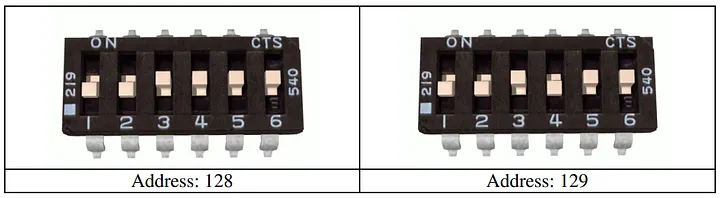
\includegraphics[width=\linewidth]{figures/photos/sabertooth_addresses_legacy.png}
\caption{Address convention retained from the previous hardware stack.}
\end{subfigure}\hfill
\begin{subfigure}{0.46\linewidth}
\centering
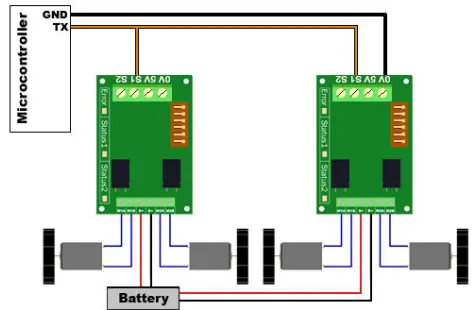
\includegraphics[width=\linewidth]{figures/photos/sabertooth_wiring_legacy.png}
\caption{Legacy Sabertooth wiring reference. Validate against the live robot before rewiring.}
\end{subfigure}
\caption{Sabertooth references retained as visual aids. RUDRAv4 uses the same addresses and single-wire packet serial principle.}
\end{figure}

\section{Why the NUC belongs at the center}

The NUC is the right place for ROS 2 because it can run the full graph, DDS discovery, LiDAR drivers, RViz networking, Python nodes, launch files, logging, and development tools. It also avoids tying robot software to microcontroller memory constraints. The microcontrollers remain excellent for deterministic low-level I/O. The NUC remains excellent for orchestration.

A practical rule follows:

\begin{operatorbox}{NUC vs. microcontroller responsibility rule}
Use the NUC for decisions that need ROS messages, parameters, launch files, sensor fusion, visualization, logs, or networking. Use the Teensy for packet serial timing, motor command ramping, encoder counting, IMU reading, and immediate command timeout. Use the Uno only for the PS2 receiver and compact joystick packet.
\end{operatorbox}

\section{USB device identity}

The robot should use persistent \filep{/dev/serial/by-id/...} device names, not short names like \filep{/dev/ttyACM0} or \filep{/dev/ttyUSB0}. Short names are assigned by probe order and can change after replugging, booting, or adding a device. Persistent names encode the USB device identity and are more stable.

Current stable paths in the workspace configuration are:

\begin{longtable}{p{0.18\linewidth}p{0.62\linewidth}p{0.13\linewidth}}
\toprule
Device & Preferred path & Typical short path\\
\midrule
Arduino Uno & \filep{/dev/serial/by-id/usb-Arduino__www.arduino.cc__0043_959313232323510182C0-if00} & \filep{/dev/ttyACM1}\\
Teensy 4.1 & \filep{/dev/serial/by-id/usb-Teensyduino_USB_Serial_9210670-if00} & \filep{/dev/ttyACM0}\\
YDLIDAR CP2102 & \filep{/dev/serial/by-id/usb-Silicon_Labs_CP2102_USB_to_UART_Bridge_Controller_0001-if00-port0} & \filep{/dev/ttyUSB0}\\
\bottomrule
\end{longtable}

Use the checked-in helper:

\begin{lstlisting}[language=bash]
cd /home/rudra/Projects/RUDRAv4
bash scripts/list_serial.sh
\end{lstlisting}

\section{Mechanical assumptions needed by software}

The software presently carries two key geometric constants from the older RUDRA design:

\begin{align}
R &= 0.0675\ \text{m} && \text{wheel radius reference},\\
L &= 0.29\ \text{m} && \text{wheelbase / track-width reference for differential motion}.
\end{align}

These values appear in the differential-drive equations, \cmd{/cmd_vel} conversion, and wheel odometry. If the physical wheel radius or track width changes, the firmware and ROS configuration must be updated together. A mismatched radius causes speed scale error. A mismatched track width causes yaw-rate error.
